\lhead[\thepage]{CHAPTER \thechapter. STATE OF THE ART}
\chead[]{}
\rhead[WepSIM: Simulador de procesador elemental con unidad de control microprogramada\leftmark]{\thepage}
\renewcommand{\headrulewidth}{0.5pt}

\lfoot[]{}
\cfoot[]{}
\rfoot[]{}
\renewcommand{\footrulewidth}{0pt}

%% This is an example first chapter.  You should put chapter/appendix that you
%% write into a separate file, and add a line \include{yourfilename} to
%% main.tex, where `yourfilename.tex' is the name of the chapter/appendix file.
%% You can process specific files by typing their names in at the 
%% \files=
%% prompt when you run the file main.tex through LaTeX.
\chapter{Estado del arte}
\label{ch:state_of_the_art}
\markboth{}{STATE OF THE ART}

Este capítulo presenta el estado del arte, la última y más avanzada etapa de las tecnologías relacionadas con nuestra aplicación. Primero, se presentan los diferentes simuladores existentes para microprogramación (Section \ref{sec:simuladores_microprogramacion}). Después, se presentan los diferentes simuladores existentes para la programación en código ensamblador (Section \ref{sec:simuladores_ensamblador}). Por último, realizamos una comparación de nuestro trabajo con el contexto actual de los distintos simuladores expuestos previamente (Section \ref{sec:propuesta_simulacion}).

\section{Simuladores para microprogramación}
\label{sec:simuladores_microprogramacion}

En esta sección, se explican los diferentes simuladores existentes para la microprogramación. En primer lugar, vamos a centrarnos en los simuladores que están más enfocados a una labor docente. 

\section{Simuladores para programación en ensamblador}
\label{sec:simuladores_ensamblador}
En esta sección, se explican los diferentes simuladores existentes para la programación en ensamblador. Los simuladores más conocidos para labores docentes, son SPIM y MARS.

SPIM \cite{larus1990spim}, es un simulador de un procesador MIPS de 32 bits que permite ejecutar programas en ensamblador para esta arquitectura. Además, también permite depurar el código implementado, de forma que el alumno pueda corregir con mayor facilidad los errores cometidos. Este simulador, fue creado por James R. Larus y tiene versiones compiladas para Windows, Mac OS X y Unix/Linux e incluso tiene una versión básica para Android, aunque su diseño no está pensado para dispositivos móviles. Puesto que el simulador está totalmente enfocado al procesador MIPS, posee el juego completo de instrucciones para la versión de 32 bits del procesador y todas las directivas de las que consta el lenguaje. Otra característica que hace de SPIM un potente simulador, es proveer de un pequeño sistema operativo que soporta las principales llamadas al sistema mediante la instrucción syscall. SPIM, es un simulador que permite múltiples configuraciones mediante su interfaz de usuario, de manera que se puede indicar:

\begin{itemize}

\item Activación del uso de pseudoinstrucciones.

\item Simulación de predicción de saltos y accesos a memoria, con la latencia correspondiente.

\item Activación del uso del manejador de la señal trap y la carga del manejador personalizado.

\item Activación de la visualización de los mensajes en caso de ocurrir excepciones.

\item Activación del uso de "memory-mapped IO".

\end{itemize}

\begin{figure}[htbp]
 	\centering
 	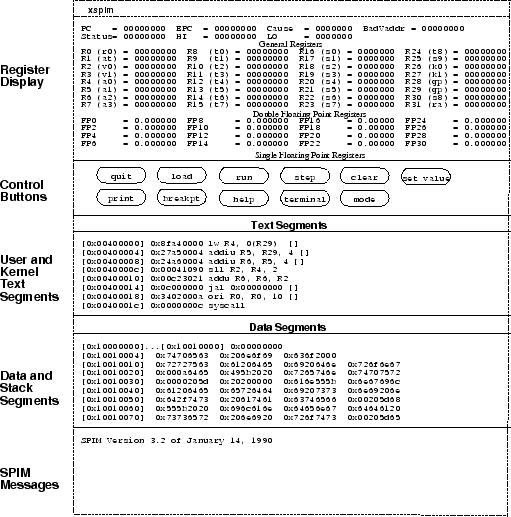
\includegraphics[width=12cm]{figures/spim_figure}
 	\caption{SPIM interface.}
	\label{fig:spim_figure}
\end{figure}

SPIM, además cuenta con una versión más actualizada del simulador, que posee una interfaz gráfica más potente. Éste simulador se llama QtSPIM \cite{aguilar2013simuladores}, y cuenta con todas las características anteriormente mencionadas de SPIM.

\begin{figure}[htbp]
 	\centering
 	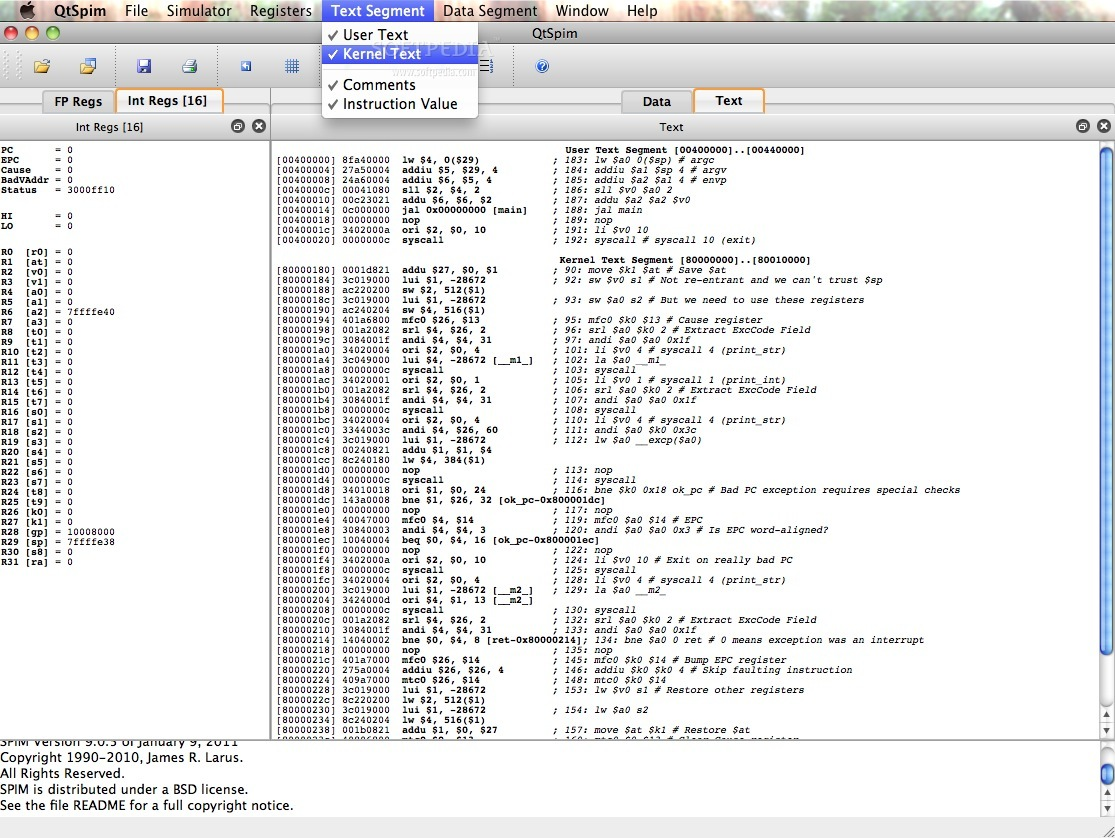
\includegraphics[width=12cm]{figures/qtspim_figure}
 	\caption{QtSPIM interface.}
	\label{fig:qtspim_figure}
\end{figure}

MARS \cite{vollmar2006mars}, es un simulador ... 

\section{Propuesta de simulación unificada}
\label{sec:propuesta_simulacion}

